\section{Case Study}

\subsection{Scenario Generation}




\subsection{Results}
Considering different values for risk aversion, we wish to compare the revenue of a hybrid producer with the revenue of single energy producer. The way we modelled the problem, it was possible to simply neglect one energy source by setting the respective parameters to zero. Apart from that, we optimised the revenue once for the situation with an adujsutment market and once for the situation without an adjustment market. The results are summarised in the figures below. 

\begin{figure}[h!]
	\centering
	
	\begin{minipage}{0.95\textwidth}
		\subfloat[]{
			\centering
			\scalebox{0.75}{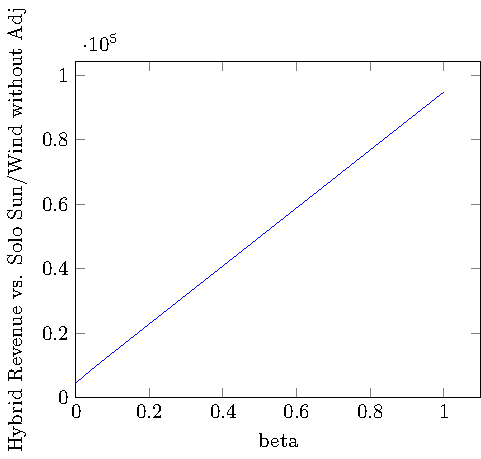
\includegraphics[]{Figures/figure2.pdf}}
		}
		\hfill
		\subfloat[]{
			\centering
			\scalebox{0.75}{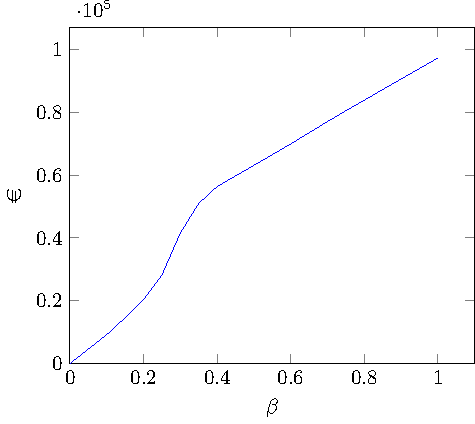
\includegraphics[]{Figures/figure.pdf}}
		}
		
		\caption{Revenue }\label{fig:overyear}
	\end{minipage}	
\end{figure}

We plotted the difference of the revenue of the hybrid producer and the sum of the revenues of both single producers on the vertical axis and presented the risk aversion factor $\beta$ on the horizontal axis. Overall, we see that the hybrid model is more advantageous for risk averse producers. The more risk averse a producer is, the more profitable it is to offer energy of both solar and wind power plants. One striking difference is that the curve on the right starts in the origin while the curve on the left does not. If we have an adjustment market and are not risk averse at all, it does not matter whether one producer offers both energies or two producers offer on energy each. The reason is that a risk seeking producer offers everything on the day-ahead market and probably buys back the deficit on the adjustment market. On the other hand, if we do not have an adjustment market, we can exploit the anti-correlation. Thus, the variance of the produced amount of energy decreases and therefore the hybrid producer can offer more energy for a given day-ahead price. Hence, it is more profitable to produce both collectively. 

Apart from that, we observe a linear growth behaviour in the case of a market system without an adjustment market. When adding the adjustment market to the system, we notice a small bump. At some value for the risk aversion factor $\beta$, the producer is not brave enough anymore to trade on arbitrage since in certain scenarios he would face losses. 